\documentclass{jlreq}

\usepackage{amsmath}
\usepackage{bm}
\usepackage{fancyhdr}
\usepackage{float}
\usepackage{graphicx}
\usepackage{physics}
\usepackage{siunitx}

\numberwithin{equation}{section}

\pagestyle{fancy}
\fancyhf{}
\fancyhead[R]{\thepage}

\begin{document}

\tableofcontents
\clearpage

\section{分析的評価の目的}
ATM\_Aの分析的評価を行い,個人の評価と班員の評価を比べることで問題点を抽出する.また,その問題点を基に具体的な解決策を考えて再設計する.

\section{実験機材}
使用した機材は,Dell\ Inspiron\ 15\ 3535である.OSはWindows11\ Homeであり,用いたR言語はR\ version\ 4.3.2である.

\section{分析的評価の方法}
銀行ATMのインターフェースのプロトタイプであるATM\_Aを実施してログを取得した.そのインターフェースを,Nelsenの10項目を基に評価した.
その後,評価内容を班員全員と共有し,問題点を炙り出した.また,問題点について考察を行い,評価をもとに要求獲得と再設計を行い,実装を行った.

\section{分析的評価の結果}
ATM\_Aの分析的評価の結果を,個人の結果は表に,班員の評価は表に示す.

\begin{table}[H]
  \centering
  \caption{ATM\_Aの分析的評価(個人)}
  \scalebox{0.5}{\begin{tabular}{|l|l|}
      \hline
      1 システムの状態を視認できるようにする                                               & ・現在位置を表示すべき                                                                   \\ \hline
      2 実環境にあったシステムを構築する(専⾨⽤語は避け,ユーザが普段使う⾔葉を使⽤する) & ~                                                                                        \\ \hline
      3 ユーザにコントロールの主導権と自由度を与える                                       & ~                                                                                        \\ \hline
      4 操作と表示に一貫性を持たせる                                                      & \begin{tabular}{l}
                                                                                               ・テンキーやかな入力は,昇順やかな順になるように一貫性を持たせて表示すべき.             \\
                                                                                               ・ボタンの色が薄かったり,濃かったり統一されていないのと,薄い表示のときに認識しづらい. \\
                                                                                               ・名前の一覧表示では,あかさたな順でそれぞれまとめた方が見やすい.                       \\
                                                                                             \end{tabular} \\ \hline
      5 フィードバックを与え、エラーの発生を事前に防止する                                 & ・振込金額を指定していなくても,フィードバックなしに確定できてしまう.                   \\ \hline
      6 記憶の負担を最小限にし、見た目だけで分かるようにする。                             & ・ボタンの色が全部一緒なので,ボタンの識別が難しい.                                     \\ \hline
      7 柔軟性と効率性を持たせる(ショートカットなど)。                                     & \begin{tabular}{l}
                                                                                               ・いくつか前の操作画面に戻るには,何回か戻るボタンを押す必要があるが, \\
                                                                                               操作画面を選択することでそのページまで飛べるようにしたい.             \\
                                                                                               ・1文字削除できる機能が欲しい.                                        \\
                                                                                             \end{tabular}                   \\ \hline
      8 余分な情報を提示しない最小限で美しいデザインにする。                               & \begin{tabular}{l}
                                                                                               金融機関名が一覧表示になっているが,「あ」から始まる金融機関名などのように, \\
                                                                                               あかさたなグループにして表示するべき.
                                                                                             \end{tabular}             \\ \hline
      9 ユーザがエラーを認識し、回復できるようにする。                                     & ~                                                                                        \\ \hline
      10 ヘルプやマニュアルを用意する。                                                    & ~                                                                                        \\ \hline
    \end{tabular}}
  \label{tab:eval_personal}
\end{table}

\begin{table}[H]
  \centering
  \caption{ATM\_Aの分析的評価(自分を除く班全員)}
  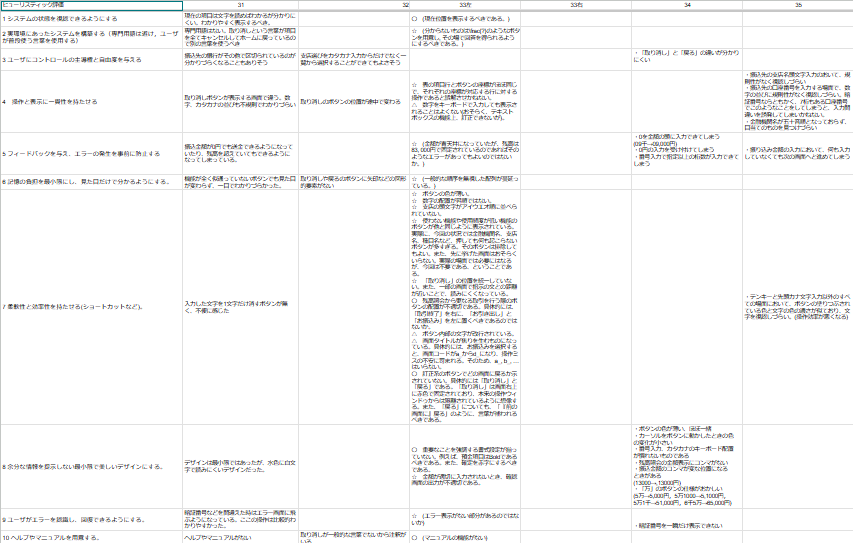
\includegraphics[width=\textwidth]{image/eval_group.png}
  \label{tab:eval_group}
\end{table}

\section{分析的評価の考察}

\section{分析的評価の考察を基にした要求仕様}

\section{設計の内容}

\begin{thebibliography}{9}
  \item 西崎友規子.プロジェクト実習Ⅰ ヒューマンインターフェース 実験テキスト.京都工芸繊維大学,2024年
\end{thebibliography}

\end{document}